\chapter{Background}

\section{概览}

概率图模型按照有向和无向分类

\begin{center}
    \begin{forest}
        forest scheme
        [概率图模型
            [有向$\rightarrow$ \textsl{Bayesian Network}]
            [无向$\rightarrow$ \textsl{Markov Random Field}]
        ]
    \end{forest}
\end{center}

概率图模型加上对时序的考量的话
\begin{center}
    \begin{forest}
        forest scheme
        [概率图模型$\rightarrow$ \textsl{Dynamic Model}
            [状态离散$\rightarrow$ \textsl{HMM}]
            [状态连续
                [Kalmen Filter]
                [Particle Filter]
            ]
        ]
    \end{forest}
\end{center}

\textsl{隐马尔可夫模型(Hidden Markov Model,HMM)}是关于时序的概率模型,描述由一个隐藏的马尔可夫链随机生成不可观测的状态随机序列,再由各个状态生成一个观测而产生观测随机序列的过程。隐藏的马尔可夫链随机生成的状态的序列,称为\textbf{状态序列};每个状态生成一个观测,而由此产生的观测的随机序列,称为\textbf{观测序列},序列的每一个位置又可以看作是一个时刻。其形式定义如下
\begin{figure}[H]
    \centering
    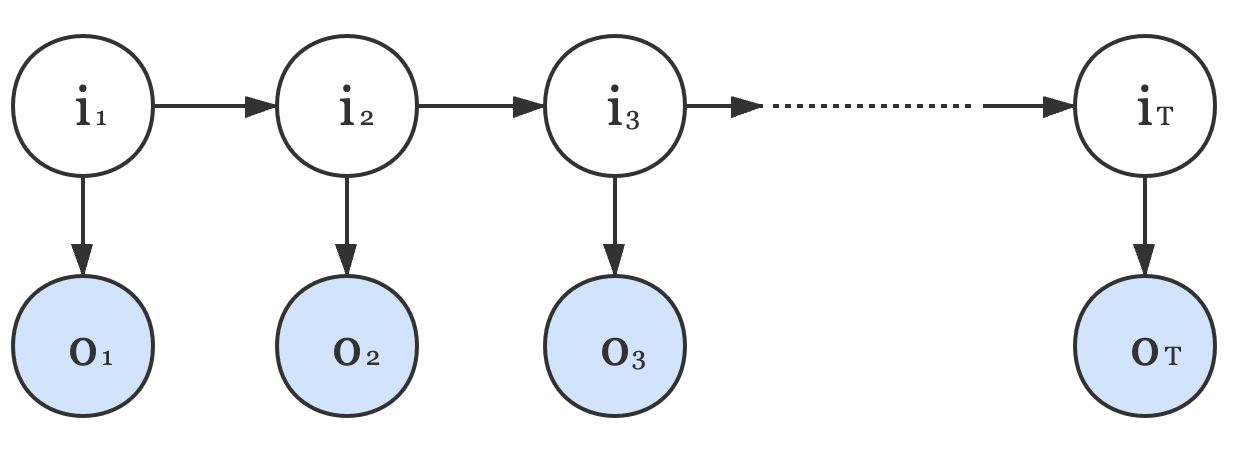
\includegraphics[scale=0.2]{figures/隐马尔可夫模型.png}
    \caption{隐马尔可夫模型,$i$是隐藏变量,$o$是观测变量}
\end{figure}

HMM可以看作是一个三元组$\lambda=(\pi,\mathcal{A},\mathcal{B})$,其中$,\mathcal{A}$是状态转移矩阵,$,\mathcal{B}$是发射矩阵。




HMM模型主是三个基本问题和两个基本假设

\begin{center}
    \begin{forest}
        forest scheme
        [三个基本问题
            [Evaluation$\rightarrow$$P(O|\lambda)$前向后向]
            [Learning$\rightarrow$$P(O|\lambda)$的$\lambda$如何求]
            [Decoding]
        ]
    \end{forest}
\end{center}
\begin{center}
    \begin{forest}
        forest scheme
        [两个基本假设
            [齐次马尔可夫假设]
            [观测独立性假设]
        ]
    \end{forest}
\end{center}

\subsection*{两个假设}

\textbf{齐次马尔可夫假设}:未来与过去无关,只和当前的状态有关,即
\begin{equation}
    P(i_{t+1}|i_t,i_{t-1},\cdots,i_1,o_t,\cdots,o_1)=P(i_{t+1}|i_t)
\end{equation}

\textbf{观测独立性假设}:观测独立性假设是指在给定隐状态序列的条件下,观测序列中的每一个观测值都是相互独立的。
\begin{equation}
    P(o_1,o_2,\cdots,o_T)=prod_{i=1}^{T}
\end{equation}





